%% This is an example first chapter.  You should put chapter/appendix that you
%% write into a separate file, and add a line \include{yourfilename} to
%% main.tex, where `yourfilename.tex' is the name of the chapter/appendix file.
%% You can process specific files by typing their names in at the 
%% \files=
%% prompt when you run the file main.tex through LaTeX.

%\makeglossaries
\newacronym{utm}{UTM}{Unmanned Aircraft System Traffic Management}
\newacronym{uav}{UAV}{Unmanned Air Vehicle}
\newacronym{uas}{UAS}{Unmanned Aircraft System}
\newacronym{nas}{NAS}{National Air Space}
\newacronym{fpv}{FPV}{First Person View}
\newacronym{vll}{VLL}{Very Low Level}
\newacronym{sme}{SME}{Small and Medium Enterprise}
\newacronym{tcas}{TCAS}{Traffic Collision Avoidance System}
\newacronym{gcs}{GCS}{Ground Control Station}
\newacronym{icao}{ICAO}{International Civil Aviation Organization}
\newacronym{faa}{FAA}{Federal Aviation Administration}
\newacronym{nasa}{NASA}{National Aeronautics and Space Administration}
\newacronym{easa}{EASA}{European Aviation Safety Agency}

\chapter{State of the Art}

\section{Fault Tolerant Control Systems}

\subsection{Terminology}\label{ch2:terminology}

Since fault tolerant control is comprised of a set of different disciplines and a relatively 
new topic, the terminology is not solid. FDI could be a proper example to this ambiguity. 
In some works, it stands for Fault Detection and Isolation while in some other 
Fault Detection and Identification, which could also named after Fault Detection and Diagnosis, 
meaning that identification is added to Fault Detection and Isolation \cite{zhang2008bibliographical}.

One of the first attempts to unify the terminology is carried out by IFAC SAFEPROCESS 
technical committee in 1996 and published by \cite{isermann1997trends}. Fault, failure, 
and the methodology to handle those such as fault detection, fault isolation, fault identification, 
fault diagnosis and supervision terms explained separately to avoid the ongoing ambiguity 
in this field. Although fault detection methods are clearer in the work, difference between 
the methods for two steps of fault diagnosis, namely the fault isolation and fault 
identification is not very obvious

\subsection{Conventions for a Safe Flight}\label{ch2:conventions}

The widely used method to increase reliability is to use more reliable components 
and/or hardware redundancy. Both requires an increase in the cost of the UAS 
conflicting one of the main reasons of UAS design itself band consumer expectations 
\cite{angelov2012sense}. To offer solutions for all different foreseen categories of 
airspace, a variety of approaches should be considered. While hardware redundancy 
could cope with the failure situations of UAVs in the certified airspace, it may not be 
suitable for UAVs in open or some subsets of specific categories due to budget 
constraints. Analytical redundancy is another solution, may be not as effective and 
simple as hardware redundancy, but relies on the design of intelligent methods to 
utilize every bit of information onboard aircraft wisely to deal with the instances.  

There are three approaches to achieve safe FTC in standard flight conventions. 
First one is the fail operational systems which are made insensitive to any single 
point component failure. The second approach is the fail safe systems where a 
controlled shut down to a safe state is practiced whenever a critical fault is pointed 
out by a sensor. The level of degradation assures to switch to robust (alternate) or 
direct (minimal level of stability augmentation independent of the nature of the fault) mode. 
Switching from nominal mode to the robust and direct modes leads to a decrease 
in the available GNC functions. This causes a degradation in ease of piloting. And 
also some optimality conditions could have been compromised. The third approach 
is fault tolerant control systems in which redundancy in the plant and the automation 
system is employed to design software that monitors the components and takes in 
action whenever needed. The strategy is most probably to try to keep plant availability 
and accept reduced performance \cite{blanke2000fault}.

RECONFIGURE project of FP7 \cite{goupil2015overview} aims to attack at this 
problem of piloting degradation and optimality compromisation by attacking 
Flight Parameter Estimation (FPE) which is the online estimation of aircraft parameters, 
FDD and FTC in case of off-nominal events \cite{RECONFIGURE} They utilize a black 
box nonlinear model of aircraft and The project uses some outputs of a previous FP 7 
project ADDSAFE leaded by Deimos Space \cite{ADDSAFE}.

\subsection{Methods for Fault Tolerant Control Systems}\label{ch1:methodsFTCS}

Among different categorizations for the fault tolerance, there are options to handle 
faults on-line or off-line. Employing fault diagnosis schemes on-line is a way to 
achieve fault tolerance. In this case, as soon as a fault detected, a supervisory 
agent is informed via a discrete event signal. Then accommodation of the faults 
are handled either with the selection of a predetermined controller for the specific 
fault case, or by designing the action online with real-time analysis and optimization \cite{blanke2000fault}.

Another common categorization of FTCS is passive and active FTCS. In passive FTCS, 
the flight controller is designed in such a way to accommodate not only the 
disturbances but also the faults. Active FTCS first distinguishes the fault via fault detection 
and diagnosis module and then switch between the designed controllers specific to the 
fault case or design a new one online \cite{angelov2012sense}. While active FTCS 
requires more tools to handle faults as seen in Fig.~\ref{fig:FTCS}, for faults 
not predicted and not counted for during the design of the robust controller, this method 
most probably fails. 

\begin{figure}
\begin{center}
%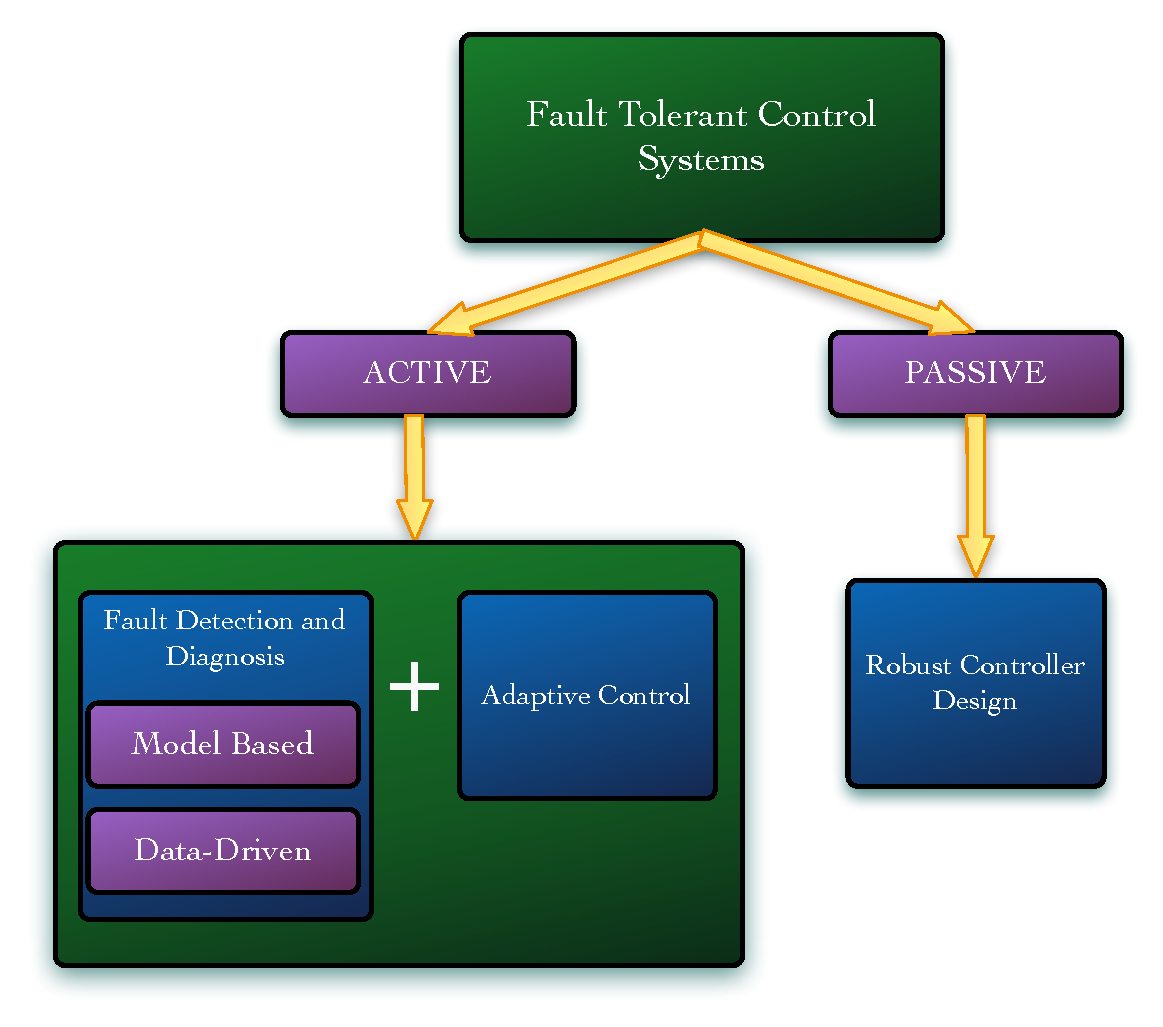
\includegraphics[width=11.3cm]{figures/FTCmethods}    % The printed column width is 8.4 cm.
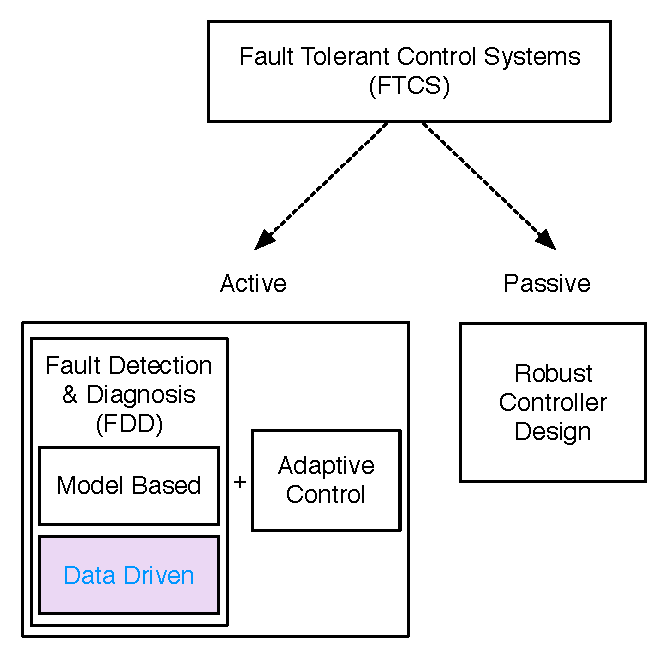
\includegraphics[width=11.3cm]{figures/FTCS}
\caption{Variations of fault tolerant control systems } 
\label{fig:FTCS}
\end{center}
\end{figure}


Even with a long list of available methods, aerospace industry has not implemented 
FTC widely, except some space systems, due to the evolving nature of the methods, 
the tricks coming with the nonlinear nature of the problem, design complexity and high 
possibility of wrong alarms in case of large disturbances and/or modeling uncertainties. 
So the already carried reliability measures concerning the hardware redundancy is 
now the preferred way because of its ease and maturity being implemented on various 
critical missions with considering human lives.

\subsection{Fault Detection and Diagnosis}

FDD is handled in two main steps; fault detection and fault diagnosis. Fault diagnosis 
encapsulates fault isolation and fault identification. The methods for detection and 
diagnosis are investigated for their frequency of utilization separately for sensor, 
actuator, process and controller faults in \cite{isermann1997trends}. FDD should 
not only be sensitive to the faults but also robust to the model uncertainties and 
external disturbances.

Two distinct options to proceed in analytical redundancy are the model based 
approaches and data-driven approaches. They form the two ends of a continuous 
solution set line, so utilizing them in a combination might end up with better solutions. 
Model based fault diagnosis highlights the components of a system and the connections 
in-between, and their corresponding fault modes. Data driven fault diagnosis rely on 
the observational data and prefers dense, redundant and with a  frequency larger than 
the failure rate. 

% This is an example of how you would use tgrind to include an example
% of source code; it is commented out in this template since the code
% example file does not exist.  To use it, you need to remove the '%' on the
% beginning of the line, and insert your own information in the call.
%
%\tagrind[htbp]{code/pmn.s.tex}{Post Multiply Normalization}{opt:pmn}

\subsubsection{Model Based Methods}

In model based approaches, relations between measurements and estimated 
states are exploited to detect possible dysfunction. The most common ways to 
implement a model based approach is to estimate the states, estimate the model 
parameters, or parity-space. The accuracy of the results depend on the type of 
faults (additive or multiplicative). Additive faults affects the variables of the process 
by a summation whereas the multiplicative faults by a multiplication.  When only 
output signal can be measured, signal model based methods can be employed for 
fault detection such as Bandpass filters, Spectral analysis(FFT) and maximum entropy estimation. 
For the case, both the input and output signals are available, the utilized methods 
for fault detection are called the process based methods: State and output 
observers(estimators), Parity equations and Identification and parameter estimation. 
They generate residuals for state variables or output variables. When previous works 
investigated, it is concluded that the most widely used technique for sensor and actuator 
faults is the state and output observers (estimators) and for process faults, identification 
and parameter estimation \cite{isermann1997trends}.

The output of the model based fault detection methods is the stochastic behaviour 
with mean values and variances. With the use of change detection methods, deviations 
from the normal behavior can be detected. For that purpose, three available methods 
considered are, mean and variance estimation, likelihood-ratio-test and Bayes decision, 
run-sum test andtwo-probe t-test. Fault detection is only supported by simple threshold 
logic or hypothesis testing in most of the applications \cite{isermann1997trends}.

A bunch of studies discovers the band of different approaches for model-based fault detection. 
Detecting sensor and actuator faults via state estimation, utilizing an EKF is applied to a 
F-16 model in \cite{hajiyev2005sensor}. Parameter identification via $H_{\infty}$ filter 
is used to indicate icing in \cite{melody2001h}.

A drawback of model-based approaches is that they require accurate model of the 
aircraft for successful detection. In a small UAV system susceptible to various 
uncertainties/disturbances and most of the cases does not have an accurate model, 
leading a model-based approach might fail. And also, a mathematical model of a UAV 
is constructed within the flight envelope, and does not necessarily describe the 
possible dynamics invoked by a failure on-board.

A way to handle that is to offer solutions to cope with the uncertainties. 
A fairly old study in 1984, investigates the design problem FDI systems robust to 
uncertainties within the models. One of the two steps of FDI, two steps being the 
residual generation and decision-making, is targeted. They offer to handle model 
uncertainties, by designing a robust residual generation process \cite{chow1984analytical}. 
Another study deals with model uncertainties by determining the threshold of the residual 
in a novel way with an application to detect aileron actuator fault \cite{rotstein2006fault}. 
\cite{sharma2007fault} utilize two cascade sliding mode observers state estimation and 
fault detection to guarantee staying in sliding manifold in the presence of unknown 
disturbances and faults. 
% This is an example of how you would use tgrind to include an example
% of source code; it is commented out in this template since the code
% example file does not exist.  To use it, you need to remove the '%' on the
% beginning of the line, and insert your own information in the call.
%
%\tgrind[htbp]{code/be.s.tex}{Block Exponent}{opt:be}

\subsubsection{Data-Driven Methods}

Model-based approaches had various successful applications until now, 
most of them assuming accurate model is available on-board. With the new 
era of UAVs, the airspace is expected to be populated by an abrupt increase 
in the number of UAVs. The variety of UAVs, expense of accurate modeling 
practices, the difficulty in modeling the behavior of UAV in case of failures, 
call for alternative approaches for the quite challenging problem of FDD. 
The increased efficiency of sensors on-board, the increase in the computational 
capabilities of autopilot processors, and the advances in machine learning 
techniques in the last decade may offer efficient data-driven solutions to FDD.

In data driven methods, a detailed knowledge about the internal dynamics 
of the system is not necessary. The data available is the source of information 
with regard to the behavior of the system. Supervised learning, which requires 
to label the fault cases previously in the training data, is usually utilized for 
data-centric inference of causes. In case of an unlabeled fault, the result is 
expected as a probability distribution of the available normal modes, identified 
fault labels and a probable unknown fault. What is needed at that point is to 
first detect and localize the fault and then to consult domain experts for labeling 
for further integration of this fault into the diagnosis scheme \cite{dataCentricDiagOffline}.

\cite{gui2002fault} argues artificial intelligent methods for fault detection of complex 
systems. Comparison between PCA and model based stochastic parity space 
approaches is given in \cite{hagenblad2004comparison}.
In \cite{li2016data}, the authors argues to use dynamic PCA since UAV flight 
controls is a dynamic system itself and DPCA can reflect unknown disturbances, 
while model-based approaches can only model typical disturbance.  


\section{Safe Integration of Drones into Airpace}
Air safety authorities are forced to develop regulations for UAS due to incidents 
disturbing public safety and demands from companies who desire to utilize them. 
There has been numerous studies, from both the FAA in US and EASA in Europe, 
but none of them decided on a regulations set for the UAVs to satisfy. Improvement 
of the reliability of the flight is considered to be one of the main obstacles for 
integrating UAVs into civil airspace. To achieve a safe flight is not an easy task 
considering the unknowns of the systems, environment and possible system faults 
and failures to emerge. To tackle the safety challenges and help the regulation 
development, NASA is currently carrying out a four years research program (up to 2019) 
to enable Unmanned aircraft traffic management solutions which are structured yet 
flexible when needed. To ensure safety, this integration needs to be achieved through 
airspace management and UAS reliability.

The preliminary airspace designs, like the one proposed by Amazon, identify different 
zones depending on the UAS capabilities, population density and altitude. Plus, 
different national rules and their progressive refinement pushes to cope with a variety 
of requirements. Open source and modular architectures are key to adapt these 
requirements. As a specific example, NASA's UTM builds, later to be refined by FAA, 
make modularity essential for UAS software to follow their evolution. 

Concerning reliability, current regulations focus on flight constraints but they might be 
expected to involve regulations on software and hardware components as well. 
In such case, the increased cost will be inevitable for the demands of certification. 
This could put too many constraints on UAS manufacturers who desire to access the G airspace. 

In Europe, Regulation (EC) No 216/2008 mandates the European Aviation Safety Agency 
to regulate Unmanned Aircraft Systems (UAS) and in particular Remotely Piloted Aircraft 
Systems (RPAS), when used for civil applications and with an operating mass of 150 Kg or more.

\section{UAVs populating airspace}\label{ch2:certificationOfAnalyticalApproaches}

The cost effectiveness and reachability of commercial off-the-shelf elements, and 
shrinking size of electronics serve as a perfect environment for small flying vehicles 
to emerge. Although inherited as military purposes in its infancy, nowadays \gls{uas} 
are becoming efficient platforms for scientific/commercial domains. They offer 
benefits in terms of cost, flexibility, endurance as well as realizing missions that 
would be impossible with a human onboard. 
Increasing usage of these vehicles for a variety of missions, such as defense, 
civilian tasks including transportation, communication, agriculture, disaster mitigation 
applications pushes demand on the airspace. Furthermore, this congestion is predicted 
to accelerate with the growing diversity of these systems. 

Commercial advantages, offered by these efficient systems, are already targeted by 
big companies worldwide, specifically in the US. The airspace regulatory authorities 
seem to be squeezed in between the companies, demanding a fast as possible 
access to airspace, and the concerns of the public about potential privacy breaches, 
safety and liability issues \cite{droneDisasters,droneImageProblem}. Even with today's 
strictly regulated airspace, reported occurrences show that there are hurdles to solve 
before a further integration of \gls{uas} to airspace.

Advent of the new era of \gls{uas} seems to be hold by an unseen barrier of lack of 
regulatory framework for now. Different institutions all over the world, specifically \gls{nasa} 
and faa in US, easa in Europe and international bases such as \gls{icao} are addressing 
safe integration of \gls{uas} in airspace. Although the approaches of regulatory bodies 
may vary, the aim remains the same: safe integration as soon as possible. 

The tackles of safety during integration of \gls{uas} to airspace refer to different technical 
and organizational aspects including but not limited to control of traffic in segregated and 
non-segregated airspace, reliable communication, robust control of the \gls{uav}, trajectory planning, detect\&avoid.


\section{Modularity}\label{ch2:modularity}

The current evolving nature of regulations and the variety of organizations in charge 
of the airspace rule making calls for flexible solutions to cope with these fruitful environments. 

\subsection{Airspace Categorization}
The \gls{uas} in the \gls{nas} project points to a performance-based routine access to 
all segments of the national airspace for all unmanned aircraft system classes, after the 
safety and technical issues are addressed thoroughly. As a start, \gls{nasa} and faa 
seem to have a short term goal to integrate \gls{uas} in low-altitude airspace as early 
as possible. They further aim to accommodate increased demand safely, efficiently in 
the long term. \gls{nasa} and faa seem to handle the airspace above 500 feet and the 
one below separately. easa, tasked by the European Union, is planning a risk based approach, 
accommodating the \gls{uas} in the airspace under three different categories, low risk, 
specific and high risk. Both regulators seem to categorize the airspace and scale regulatory 
needs according to some criteria. To answer different needs of different categories, flexibility 
given by the high level of modularity of open source autopilot systems will be a handy tool. 

\subsection{National Regulations}
Circulation of \gls{uas} internationally is somewhat prevented by the Chicago convention 
unless an agreement holds between Contracting States \cite{A_NPA_EASA2015}. \gls{icao} is aiming 
to develop international standards and recommended practices to which the member states 
could refer to when developing their national civil aviation regulations. Even though a similar 
base is aimed, national aviation legislations will not be the same because of the different 
expectations of nations about \gls{uas} aviation. 

\subsection{Accommodating evolution of regulations}
Prescriptive rules seem to cause some difficulties since the technical area on \gls{uas} 
systems develop rapidly \cite{A_NPA_EASA2015}. Innovations both on the aircraft and the operation 
type of \gls{uas} will accelerate especially after the regulations are set. Thus, regulatory 
bodies call for refinable operational requirements and system architectures to evolve into 
a safer and efficient integration of \gls{uas} into airspace. The systems to cope with the 
regulations should also be modular and flexible in order not to be superseded by the 
innovations in the area. 
Thus, the aviation regulatory bodies aim to achieve designs with flexibility where possible, 
structure where needed. Having flexible hardware and software points to modularity, which 
is pretty much best supported via open source systems.



\section{Congestion management}\label{ch2:congestion}

According to \textit{UAV Factory}, one of the large European \gls{uas} companies, 
``The future of the UAV industry is likely to be shaped by airspace congestion'' 
\cite{europe_report_civilian_drone}. Indeed, high level airspaces are getting crowded 
and large scale solutions, such as NextGen (US) or SESAR-JU (EU), are necessary to 
increase airspace capacity while maintaining the current safety levels. However, there is 
no such management solution existing for \gls{vll}. Yet, large projects like Amazon's 
Prime Air and Google's Project Wing are already waiting to populate the \gls{vll} airspace.	
	
Part of the congestion management problem is to avoid conflicts, and more importantly 
collisions, between \gls{uas} through strategic deconfliction and safety nets.
Another mission of the congestion management system is to make sure that \gls{uas} 
do not go where they are not supposed to go, thus requiring geofencing. In order to implement 
the previously mentioned systems, the \gls{uas} autopilot needs to be able to perform complex 
operations, e.g. static waypoints following is likely to be insufficient.

In the following, we divide these issues into four topics of interest: 4-D trajectory management, 
geofencing, safety nets, complex operations.
	
\subsection{4-D Trajectory Management}
As noted in \cite{erzberger_4D_2002}, 4-D trajectories will be central in future airspace 
management methods. The principle of 4-D trajectory management is to have every 
\gls{uas} broadcast its trajectory up to some time horizon and receive \gls{utm}'s 
clearances under the form of trajectories. The trajectory information contains a path, 
the series of points through which the \gls{uas} will pass, and times associated to each of these points. 
Thanks to this information, the idea is to perform pro-active deconfliction, as 
explained by Thomas et al. in \cite{thomas_4D_2015}. In clear, it implies that \gls{utm} 
detects future conflicts along the trajectories of all \gls{uas} and deconflicting them 
as safely and early as possible. 
				
\subsection{Safety Nets}
Trajectory deconfliction is the first step to manage congestion, however safety nets 
are also part of the congestion management. Indeed, safety nets such as self-separation 
and collision avoidance allow \gls{uas} to fly close to each other while preserving an 
acceptable safety level.
		
\subsection{Geofencing}
Keeping \gls{uas} away from each other is an important point. But keeping them 
out of forbidden areas is also crucial. Geofencing allows determining no-fly zones 
where the \gls{uas} should not enter.

To accommodate land owners while managing traffic and limiting congestion, Foina et al. 
\cite{foina_air_parcelle_2015} proposed a participative dynamical airspace management 
method: the air-parcel model. It allows land owners to authorize/forbid flights over their 
lands through a web interface. However, this type of approach asks from the \gls{uas}s 
to be able to handle dynamical geofencing. Plus, though initially this model considers only 
cuboid parcels, the need for more precise airspace shapes may emerge making 3-D geofencing a need.
	
\subsection{Complex Operations}
Having 4-D trajectory management, safety nets and geofencing is useless if the \gls{uas}s 
cannot follow the instruction from \gls{utm} regarding these tools. Indeed, new \gls{utm} 
paradigms imply being able to change flight plans dynamically to answer to \gls{utm} demands. 
In \cite{wargo_complex_2015} two types of complex operations examples are mentioned: 
space transition corridors and temporary flight restriction. Both these airspace management 
methods require from the \gls{uas} to be able to modify its flight plan according to new \gls{utm} instructions.
		

\section{Reliability}\label{ch2:reliability}

Improvement of the reliability of the flight is considered to be one of the main goals for 
integrating military \gls{uav}s into civil airspace according to Unmanned systems roadmap 
by US Office of the Secretary of Defense, DoD \cite{UnmannedSystemsRoadmapDoD}. 
Compared to manned counterparts, \gls{uav}s experienced failures with a frequency of two 
orders of magnitude more in the military domain.  Although this changed last years with 
the technological improvements, making the \gls{uav}s as reliable as early manned military 
aircraft, it seems not enough from the DoD perspective. This can be realized by checking 
the biggest chunk of control technologies budget for research and development, which is 
health management and adaptive control.

To achieve a safe flight is not an easy task considering the unknowns of the systems hardware, 
environment and possible system faults and failures to emerge. Also, increasing demand on 
cost effective systems, resulting in smaller sensors and actuators with less accuracy, 
impose the software to achieve even more. The expectation that \gls{uav}s should be less 
expensive than their manned counterparts might have a hit on reliability of the systems. 
Cost saving measures other than the need to support a pilot/crew onboard or decrement 
in size would probably lead to decrease in system reliability. 

\subsection{\gls{sme}s and Certification Costs}

Utilizing drones for quicker and cheaper deliveries could be rewarding for \gls{sme}s 
since cost per mile of a drone is less then 1 / 30 of the average diesel truck. Being an 
early bird might put the \gls{sme}s in an advantageous position, considering the increase 
in the capabilities of the drones with inevitable acceleration thrusted by research activities 
and their widened application areas. 

Nevertheless, the fairly cheap access to drones and their relatively cheap utilization cost 
does not seem to be enough to put them to air right now due to the heavy cost of certification 
and regulatory hurdles \cite{UAVreliabilityStudy}. In this concern, capable open source solutions 
could be a good way to loosen the tie.  Otherwise, \gls{sme}s, an important factor in drone 
business might not survive. Even worse, they might operate them without relevant permission, 
scarifying a substantial fine as reported by Civil Aviation Authority (CAA). This will compromise 
security in the system contradicting the hopes for reliable integration of drones into airspace. 

\subsection{Individuals and Education}

Individuals, as well as \gls{sme}s, suffer from the same budget constraints. Personal \gls{uav} 
usage counts for a substantial amount of the drone ecosystem.  Both US and European 
authorities mention the importance of individuals in utilizations of drones. There is a community 
with a passion of aviation and potential, but most probably not very experienced.  

\subsection{Flight Heritage for Risk Assessment}

Drone industry being extremely innovative, technical developments could supersede the 
prescriptive rules as regulations. Thus a solution might be to follow a risk based approach 
rather that to have strict rules to cope with. Predicted regulations in Europe seems to evolve 
under different categories dedicated to specific operation risks. Flight heritage and occurrence 
reporting is expected to be an inevitable part of safety risk assessment to achieve reliable flight. 

\subsection{Support for real time planning and onboard vehicle automation}
To access low-altitude airspace with the use of small unmanned aircraft safely, an important 
ability could be to implement real-time planning and on-board vehicle automation. Amazon 
offers that this approach will allow some flexibility to adapt to variable situations such as 
weather changes, severe winds or any other emergency needs.

To conclude, the introduction of \gls{uas}s in the \gls{vll} airspace comes with numerous challenges. 
Though various ways to address them have been proposed, there is still no certainty about how it will be done in the end.

One sure thing is that it will involve two main actors: \gls{utm} and \gls{uas}s. This work focused on the later.	

\section{Certification of analytical approaches NOT FINISHED }\label{ch2:certificationOfAnalyticalApproaches}


Due to the lack of the modeling for interaction in-between different FPE  (Flight Parameter Estimation), FDD and FTC modules in simulations, leaves them free from practical limitations, offering a long way to go for these analytical methods to be certified. 

[REF : certificationOfFDD]
[REF : clearanceOptimBased]


safety issues

http://www.techrepublic.com/article/12-drone-disasters-that-show-why-the-faa-hates-drones/

%FP7_RECONFIGURE REF : FP7RECONFIGUREgeneral page : 978 starting with 4 980 section 4. VERIFICATION AND VALIDATION

Regulations EU : https://easa.europa.eu/unmanned-aircraft-systems-uas-and-remotely-piloted-aircraft-systems-rpas

The increased cost will be inevitable for the demands of certification. REF : UAVreliabilityStudy

This increment could be even beyond expectations that it could lead to a cancellation of project:  REF : http://www.defenseindustrydaily.com/euro-hawk-program-cleared-for-takeoff-03051/

Regulations US : 

US Delivery Drones (News from Guardian http://www.theguardian.com/technology/2015/nov/06/alphabet-and-facebook-compete-with-secret-drone-plans)
--------------------
Even if the companies solve the technical challenges of keeping drones aloft for long periods, sharing data via lasers and serving city-sized areas, both Alphabet and Facebook still face regulatory hurdles. Neither company has been granted a waiver to the current FAA blanket ban on the commercial operation of unmanned aircraft.

Alphabet has applied for an exemption, called ?333? after a section of the FAA regulations, for its Project Wing delivery drones, but that is yet to be granted and in any case would only clear operation to a maximum height of 400ft. Google has also been testing its delivery drones in the US under a Certificate of Waiver or Authorization (COA) with Nasa, which permitted flights intended to help Nasa develop an automated air traffic control system for low-flying drones. This would not apply to drones flying far above other manned and unmanned aircraft.

?There?s not a lot to run into between 60,000 and 90,000 feet,? says Cummings. ?But I?m sure regulators would be deeply suspicious if Google and Facebook were flying these over the US.?

Facebook and Alphabet would not comment.

What's really standing in the way of drone delivery?
---------------------------------------------------------
http://www.theverge.com/2016/1/16/10777144/delivery-drones-regulations-safety-faa-autonomous-flight


 SORASORA SORA SORA Fig.~\ref{fig:sora_barriersSmallerVersion}
\begin{figure}
\begin{center}
\includegraphics[width=24cm,angle=90,origin=c]{figures/sora_barriersSmallerVersion}    % The printed column width is 8.4 cm.
\caption{SORA structure: threats, threat barriers, hazard, harm barriers, harms} 
\label{fig:sora_barriersSmallerVersion}
\end{center}
\end{figure}

